\chapter{Tidskompleksitet}\label{chap:ch14}

Når vi diskuterer en algoritmes effektivitet, vil vi gerne forstå, hvordan den skalerer med inputstørrelsen, uafhængigt af detaljer om bestemt hardware eller bestemte programmeringsmiljøer. \textit{Teoretisk} tidskompleksitet, som almindeligvis udtrykkes med store $\mathcal{O}$-notation (med et stort $\mathcal{O}$, ikke et nul), muliggør denne abstraktion ved at fokusere på de dominerende led i algoritmens opførsel, når inputtet bliver stort. Notationen, som også kaldes Landaus symbol, blev indført af den tyske talteoretiker Edmund Landau. Her står $\mathcal{O}$ for »orden« (engelsk »order«) og indfanger en funktions vækstrate.

I dette kapitel introducerer vi de værktøjer, der skal til for at analysere algoritmers effektivitet med notationerne store $\mathcal{O}$, Omega ($\Omega$) og Theta ($\Theta$).\footnote{I praksis bruges store $\mathcal{O}$ ofte uformelt som en paraplybetegnelse, når man taler om asymptotisk analyse i almindelighed, men teknisk set omfatter den ikke $\Theta$ eller $\Omega$. Hver notation har sit eget specifikke anvendelsesområde, idet den afgrænser funktionens vækstrate fra forskellige perspektiver (øvre, nedre og stramme grænser), som vi snart skal se.}

\section{Introduktion til kompleksitetsanalyse}\label{sec:ch10sec1}

En analyse af en algoritme kan for eksempel vise, at den tid, det tager at løse et problem af størrelse $n$, er givet ved $T(n)=4 n^2-2 n+2$. Ved at se bort fra konstanter -- da de varierer med hardwaren -- og fra langsommere voksende led forenkler vi dette til $T(n)=\mathcal{O}\left(n^2\right)$ og fremhæver dermed det dominerende led. Denne abstraktion hjælper os med at forstå kompleksiteten for store input uafhængigt af det konkrete miljø, og det gør store $\mathcal{O}$ til et stærkt værktøj til at sammenligne algoritmer.

De to centrale elementer i denne teoretiske abstraktion er:

\begin{enumerate}
    \item \textbf{Vi ser bort fra multiplikative konstanter:} Konstanter afhænger ofte af faktorer som processorhastighed eller compileroptimeringer, hvilket gør dem upraktiske i en generel analyse.
    \item \textbf{Vi fokuserer på den asymptotiske opførsel:} Vi koncentrerer os om algoritmens opførsel for store input, da små tilfælde typisk kører hurtigt på enhver moderne maskine.
\end{enumerate}

I \textit{praktisk} tidskompleksitet spiller hvert led derimod en rolle -- også konstanterne. Når koden køres på bestemt hardware i et kendt miljø, kan de »ubetydelige« konstanter i store $\mathcal{O}$ blive betydelige, især for algoritmer, der anvendes på små og mellemstore datasæt. Store $\mathcal{O}$ er altså afgørende for analyse på et overordnet niveau og for sammenligning af algoritmer, men i praksis kræver kompleksiteten ofte, at man ser på hvert eneste led i kompleksitetsudtrykket. Det følgende eksempel illustrerer dette.

\begin{lstlisting}[style=pythonStyle, caption={Lineær søgning i Python}, label={lst:python_linear_search}]
    def linear_search(arr, target):
        for i in range(len(arr)):
            if arr[i] == target:
                return i
        return -1
\end{lstlisting} \newpage
    
% Use Java style for a Java code listing
\begin{lstlisting}[style=javaStyle, caption={Lineær søgning i Java}, label={lst:java_linear_search}]
    public static int linearSearch(int[] arr, int target) {
        for (int i = 0; i < arr.length; i++) {
            if (arr[i] == target) {
                return i;
            }
        }
        return -1;
    }
\end{lstlisting}

Koden udfører en lineær søgning gennem en liste og kontrollerer hvert element, indtil den finder målet eller når listens slutning. Her er tidskompleksiteten $\mathcal{O}(n)$ i værste tilfælde, da alle elementer skal kontrolleres. For små lister kan forskellen være ubetydelig, men når inputstørrelsen vokser, bliver den lineære sammenhæng mellem inputstørrelse og køretid tydelig.

Når vi spørger »Hvor effektiv er en algoritme eller et stykke kode?«, skal vi være opmærksomme på, at effektivitet omfatter forskellige ressourcer, herunder:
\begin{itemize}
    \item CPU-forbrug (tid)
    \item Hukommelsesforbrug
    \item Diskforbrug
    \item Netværksforbrug
\end{itemize}

Alle disse ressourcer er vigtige, men i dette kapitel fokuserer vi primært på tidskompleksitet, som vedrører CPU-forbruget.

\begin{enumerate}
    \item \textbf{Ydeevne:} Dette angiver, hvor meget tid, hukommelse, diskplads eller andre ressourcer der faktisk bruges, når et program køres. Ud over selve koden påvirkes ydeevnen af faktorer som maskinen, compileren, kørselsmiljøet og andre implementeringsdetaljer.
    \item \textbf{Kompleksitet:} Kompleksitet beskriver derimod, hvordan et programs eller en algoritmes ressourcebehov skalerer med størrelsen af det problem, der skal løses. Kompleksitetsanalyse fokuserer på de teoretiske aspekter af en algoritmes ydeevne og karakteriserer, hvordan ressourceforbruget vokser, når inputstørrelsen øges.
\end{enumerate}

Kompleksitet påvirker ydeevnen, men ydeevnen alene giver ikke et fuldstændigt billede af en algoritmes effektivitet med hensyn til skalerbarhed. Det er afgørende at forstå begge dele for at kunne vurdere, hvor godt en algoritme vil klare sig i forskellige virkelige scenarier, især når inputstørrelserne vokser betydeligt.

\section{Funktioners vækst}
I \autoref{sec:ch10sec1} bemærkede vi, at store $\mathcal{O}$-notation fokuserer på det dominerende led i en algoritmes tidskompleksitet og abstraherer konstanter og mindre led væk. Denne forenkling bygger på den idé, at det dominerende led bestemmer algoritmens kompleksitet, når inputstørrelserne bliver store. Se på følgende Java-kodestykke:

\newpage

\begin{lstlisting}[style=javaStyle, caption={SumCalculator i Java}, label={lst:java_f_function}]
    public static int f(int n) {
        int sum = 0;
        for (int i = 0; i < n; i++) {
            for (int j = 0; j < n; j++) {
                sum += (i + j) / 6;
            }
        }
        return sum;
    }
\end{lstlisting}

Koden ovenfor er en implementering af følgende udtryk:

\[
\operatorname{sum}=\sum_{i=0}^{n-1} \sum_{j=0}^{n-1} \frac{i+j}{6}
\]

Antag, at $n$ er et ikkenegativt heltal, og lad $T(n)$ betegne den CPU-tid, en typisk bærbar computer bruger på at udføre funktionen\footnote{I Java er det teknisk set en metode, ikke en funktion. I Javas terminologi kaldes en funktion, der tilhører en klasse (funktionen ville formentlig tilhøre en klasse som \inlinecode{public class SumCalculator}), en metode. En funktion betegner generelt en selvstændig kodeblok, der kan kaldes uafhængigt, hvilket er typisk i sprog som C eller Python.}  $f(n)$ med input $n$. $T(n)$ kan naturligvis variere på grund af faktorer, som vi ikke fuldt ud har kontrol over, såsom den specifikke Java-compiler, den bærbare computers hardwarespecifikationer, styresystemet og andre programmer, der kører samtidig. Vi kan dog være sikre på løkkernes struktur: Den ydre løkke kører $n$ gange, og for hvert gennemløb af den ydre løkke kører den indre løkke også $n$ gange, hvilket giver i alt $n^2$ iterationer. 

Hver iteration kræver et omtrent konstant antal clockcyklusser, betegnet \( c \), som kan variere fra system til system. I stedet for at sige, at »$T(n)$ er omtrent \( cn^2 \) nanosekunder for en konstant \( c \), der varierer mellem systemer«, bruger vi store $\mathcal{O}$-notation og skriver \( T(n) = \mathcal{O}(n^2) \). Notationen udtrykker, at CPU-tiden højst vokser kvadratisk med \( n \). For at gøre det anskueligt kan vi se på en graf af \( T(n) \), som generelt vil være parabelformet med den omtrentlige form \( cn^2 \), hvor \( c > 0 \) er en konstant.

\begin{figure}[htbp]
    \centering
    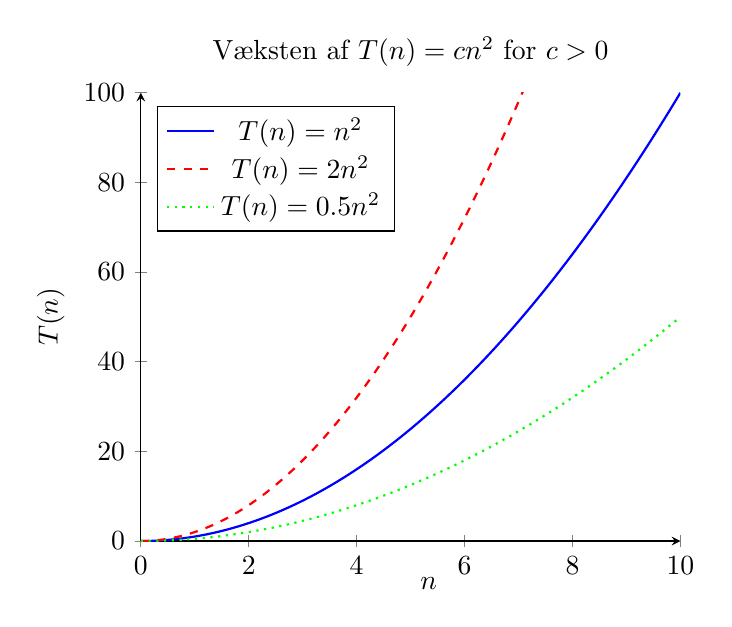
\begin{tikzpicture}
        \begin{axis}[
            domain=0:10,
            samples=100,
            axis lines=left,
            xlabel={$n$},
            ylabel={$T(n)$},
            ymin=0, ymax=100,
            xmin=0, xmax=10,
            xtick={0,2,4,6,8,10},
            ytick={0,20,40,60,80,100},
            xlabel style={right},
            ylabel style={above},
            legend pos=north west,
            title={Væksten af $T(n) = cn^2$ for $c > 0$}
        ]
            \addplot[blue, thick] {x^2};
            \addlegendentry{$T(n) = n^2$}

            \addplot[red, thick, dashed] {2*x^2};
            \addlegendentry{$T(n) = 2n^2$}

            \addplot[green, thick, dotted] {0.5*x^2};
            \addlegendentry{$T(n) = 0.5n^2$}
        \end{axis}
    \end{tikzpicture}
    \caption{Graf af $T(n) = cn^2$, der illustrerer kvadratisk vækst for forskellige værdier af $c$}
    \label{fig:quadratic_growth}
\end{figure}

Store $\mathcal{O}$-notation gør det muligt at se bort fra konstanter, som ofte varierer og ligger uden for vores kontrol, men som ikke påvirker funktionens »familie«, dvs. den overordnede klassificering af dens vækstrate. For eksempel tilhører enhver mulig funktion $T(n)$ i dette tilfælde familien af andengradsfunktioner, som illustreret i figur \ref{fig:quadratic_growth}. Desuden bliver led af lavere orden ubetydelige for store $n$, da de kan begrænses af et konstant multiplum af det dominerende led. 

Hvis for eksempel $f(n) = 3.5n^2 + 4n + 36$, ser vi, at $f(n) \geq 3.5n^2$. Samtidig gælder

\[
f(n) = 3.5n^2 + 4n + 36 \leq 3.5n^2 + 4n^2 + 36n^2 = 43.5n^2,
\]

hvilket reelt »klemmer« $f(n)$ inde mellem to andengradsfunktioner og bekræfter, at dens vækst i det væsentlige er kvadratisk.

\subsection*{Grundlæggende funktioner}
For at forstå, hvordan funktioner vokser, ordner vi nogle grundlæggende funktioner efter deres vækstrate. Vi leder efter relationer på formen \( f(n) \leq g(n) \), men da vi kun interesserer os for opførslen for store input, gælder disse relationer kun over en vis nedre grænse \( k \) for \( n \).

Lad os begynde med det grundlæggende: Enhver konstant funktion vokser langsommere end en lineær funktion, simpelthen fordi en konstant slet ikke vokser. For tilstrækkeligt store værdier vokser en lineær funktion langsommere end en andengradsfunktion, mens en tredjegradsfunktion vokser hurtigere end en andengradsfunktion.

Eksponentialfunktioner er velkendte for deres hurtige vækst. Tænk på historien om en virksomhed, der besluttede at belønne en medarbejder ved at fordoble vedkommendes bonus hver dag i en måned. Selv om det begyndte med et beskedent beløb, eskalerede den eksponentielle stigning hurtigt, og ved månedens udgang ville bonussen være astronomisk. Da virksomheden indså, at omkostningerne var uholdbare, ændrede den hurtigt aftalen til et fast beløb i stedet. Matematisk er effekten tydelig: \( n^2 < 2^n \) for ethvert heltal \( n \geq 5 \). Mere generelt gælder \( n^k < 2^n \) for enhver eksponent \( k \), når \( n \) er tilstrækkeligt stor.

Endnu mere dramatisk er fakultetsvækst, repræsenteret ved \( n! \), som overhaler eksponentiel vækst for store \( n \). Begrundelsen er, at \( 2^n \) består af \( n \) faktorer 2, mens \( n! \) har de første \( n \) heltal som faktorer, og de fleste af dem er større end 2. Derfor vokser \( n! \) til sidst hurtigere end \( 2^n \). 

Sammenfattende er eksponentiel vækst hurtigere end enhver polynomiel vækst, og fakultetsvækst overgår dem begge. Med \(1\) som vores konstante funktion kan vi udtrykke disse relationer som:

\[
1 \prec n \prec n^2 \prec n^3 \ldots \prec 2^n \prec n!
\]

Symbolet \( \prec \) bruges her, fordi denne ordning ikke er en almindelig algebraisk ulighed og kun gælder, når \( n \) er tilstrækkeligt stor.

Ved design af computerprogrammer er kun de første få af disse vækstrater praktisk anvendelige. Tredjegradspolynomier kan allerede vokse for hurtigt for større input, og algoritmer med eksponentiel køretid er kun brugbare i meget små tilfælde. Eksponentielle algoritmer erstattes ofte af hurtigere, approksimative metoder som statistisk stikprøveudtagning.

Lad os nu se på funktioner med langsommere vækst -- det er den type funktioner, vi stræber efter i effektive algoritmer. Algoritmer til søgning i store datasæt har ofte køretider, der er proportionale med \( \log n \). Hvis vi plotter \( \log n \) for værdier større end 1, ses en langsom, men stabil vækst, som er meget langsommere end væksten af \( n \) selv.

\begin{figure}[htbp]
    \centering
    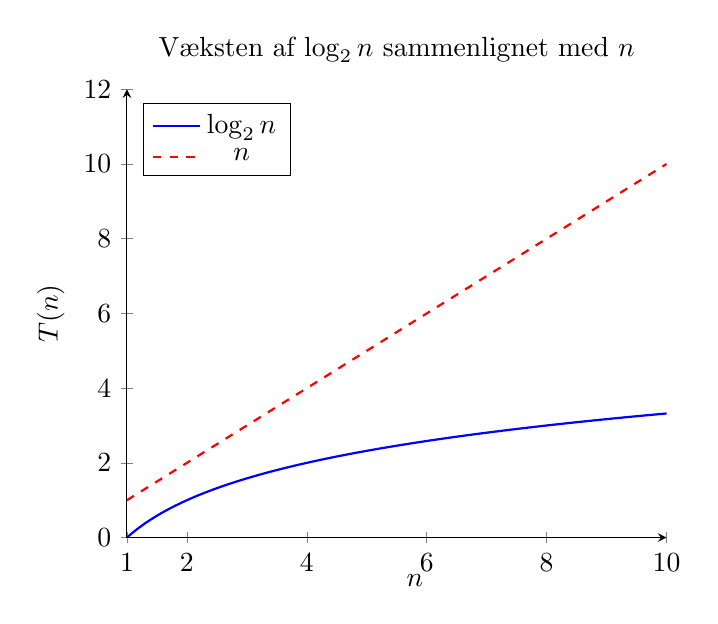
\begin{tikzpicture}
        \begin{axis}[
            domain=1:10,
            samples=100,
            axis lines=left,
            xlabel={$n$},
            ylabel={$T(n)$},
            ymin=0, ymax=12,
            xmin=1, xmax=10,
            xtick={1,2,4,6,8,10},
            ytick={0,2,4,6,8,10,12},
            xlabel style={right},
            ylabel style={above},
            legend pos=north west,
            title={Væksten af $\log_2 n$ sammenlignet med $n$}
        ]
            % Plot for log(n)
            \addplot[blue, thick] {ln(x)/ln(2)};
            \addlegendentry{$\log_2 n$}

            % Plot for n
            \addplot[red, thick, dashed] {x};
            \addlegendentry{$n$}
        \end{axis}
    \end{tikzpicture}
    \caption{Graf, der sammenligner vækstraterne for $\log_2 n$ og $n$}
\end{figure}

Sorteringsalgoritmer har derimod ofte køretider, der er proportionale med \( n \log n \). For store \( n \) ser vi, at \( 1 < \log n < n \), hvilket fører til \( n < n \log n < n^2 \). Denne rækkefølge kan sammenfattes som:

\[
1 \prec \log n \prec n \prec n \log n \prec n^2
\]

\begin{remark}
    Når vi skriver $\log n$, mener vi typisk logaritmen med grundtal 2, da den er den mest almindelige inden for datalogi og softwareudvikling. Logaritmens grundtal påvirker dog ikke vækstraten, da det kun tilføjer en konstant faktor. For eksempel vokser $\log_2 n$ og $\log_{10} n$ lige hurtigt og adskiller sig kun ved et konstant multiplum.
\end{remark}

\begin{table}[htbp]
    \centering
    \renewcommand{\arraystretch}{1.4}
    \begin{tabular}{|c|l|l|}
        \hline
        \textbf{Kompleksitet} & \textbf{Vækstrate} & \textbf{Eksempler på algoritmer} \\
        \hline
        \( \mathcal{O}(1) \) & Konstant & Opslag af et element i et array \\
        \hline
        \( \mathcal{O}(\log n) \) & Logaritmisk & Binær søgning \\
        \hline
        \( \mathcal{O}(n) \) & Lineær & Lineær søgning \\
        \hline
        \( \mathcal{O}(n \log n) \) & Linearitmisk (eller log-lineær) & MergeSort, HeapSort, QuickSort (forventet) \\
        \hline
        \( \mathcal{O}(n^2) \) & Kvadratisk & Bubble Sort, Selection Sort \\
        \hline
        \( \mathcal{O}(n^3) \) & Kubisk & Matrixmultiplikation \\
        \hline
        \( \mathcal{O}(n^k) \) & Polynomiel & Approksimationsalgoritmer i polynomiel tid \\
        \hline
        \( \mathcal{O}(c^n) \) & Eksponentiel & Subset sum, brute force til kombinatoriske problemer \\
        \hline
        \( \mathcal{O}(n!) \) & Fakultet & Brute force til den handelsrejsendes problem \\
        \hline
        \( \mathcal{O}(n^n) \) & Supereksponentiel & Rekursive algoritmer med høj forgreningsgrad \\
        \hline
    \end{tabular}
    \caption{Vækstrater for almindelige funktioner og eksempler på algoritmer}
    \label{tab:growth_rates}
\end{table}


Tabel \ref{tab:growth_rates} sammenfatter vækstraterne for almindelige funktioner og giver eksempler på algoritmer med disse vækstrater, og figur \ref{fig:time_complexities} giver en visuel fremstilling af dem. Det er værdifuldt at lære den indbyrdes rækkefølge af disse almindelige funktioner udenad, da de vil dukke op igen mange gange i dette kapitel og i andre sammenhænge inden for softwareudvikling.

\begin{figure}[htbp]
    \centering
    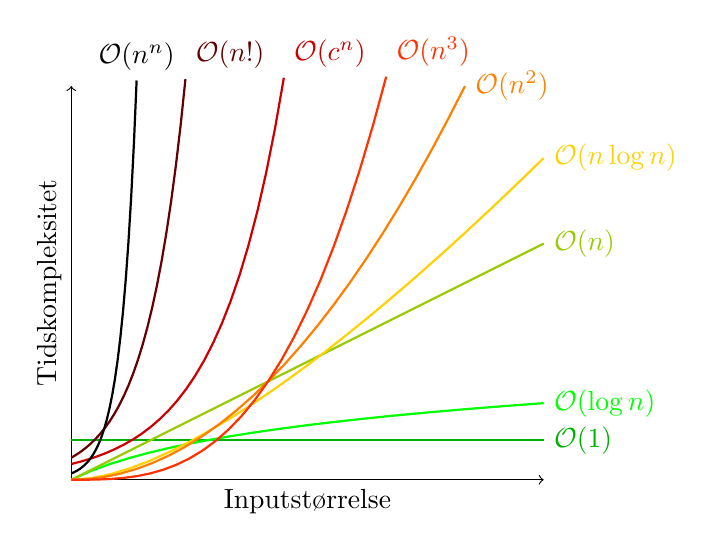
\begin{tikzpicture}
        % Draw axes
        \draw[->] (0,0) -- (0,5) node[midway, rotate = 90, anchor = south] {Tidskompleksitet};
        \draw[->] (0,0) -- (6,0) node[below, midway] {Inputstørrelse};

        % Draw conceptual growth curves
        \draw[thick, green!70!black] plot [domain=0:6] (\x, {0.5}) node[right] {$\mathcal{O}(1)$};
        \draw[thick, green] plot [domain=0:6] (\x, {0.5*ln(\x+1)}) node[right] {$\mathcal{O}(\log n)$};
        \draw[thick, lime!80!black] plot [domain=0:6] (\x, {0.5*\x}) node[right] {$\mathcal{O}(n)$};
        \draw[thick, yellow!70!orange] plot [domain=0:6] (\x, {0.35*\x*ln(\x+1)}) node[right] {$\mathcal{O}(n \log n)$};
        \draw[thick, orange] plot [domain=0:5] (\x, {0.2*\x^2}) node[right] {$\mathcal{O}(n^2)$};
        \draw[thick, red!60!orange] plot [domain=0:4] (\x, {0.08*\x^3}) node[above right] {$\mathcal{O}(n^3)$};
        
        % Make O(2^n) and O(n!) much steeper
        \draw[thick, red!80!black] plot [domain=0:2.7] (\x, {0.2*exp(\x*1.2)}) node[above right] {$\mathcal{O}(c^n)$};
        \draw[thick, red!40!black] plot [domain=0:1.45] (\x, {0.28*exp(\x*2)}) node[above right] {$\mathcal{O}(n!)$};
        \draw[thick, black] plot [domain=0:0.83] (\x, {0.08*exp(\x*5)}) node[above] {$\mathcal{O}(n^n)$};

    \end{tikzpicture}
    \caption{Begrebsmæssig illustration af tidskompleksiteter}
    \label{fig:time_complexities}
\end{figure}

I næste afsnit introducerer vi notationerne store $\mathcal{O}$, Omega ($\Omega$) og Theta ($\Theta$), som beskriver henholdsvis øvre, nedre og stramme asymptotiske grænser. Notationerne kan anvendes på enhver valgt køretidsfunktion. Køretiderne i bedste, gennemsnitlige og værste tilfælde er separate funktioner, og hver af dem kan afgrænses med en hvilken som helst af de tre notationer.


\section{Asymptotisk analyse}
I algoritmeanalyse beskriver notationerne store $\mathcal{O}$, Omega ($\Omega$) og Theta ($\Theta$) asymptotiske grænser for en bestemt funktion, fx køretiden i værste tilfælde $T_{\mathrm{worst}}(n)$ eller den forventede køretid $T_{\mathrm{avg}}(n)$. Vi kan generelt følge denne systematiske fremgangsmåde:

\begin{enumerate}
    \item \textbf{Identificér de dominerende operationer:} Fokusér på de operationer, der bidrager mest til køretiden, især dem, der vokser hurtigst, når inputstørrelsen øges.
    
    \item \textbf{Se bort fra konstanter og led af lavere orden:} I store $\mathcal{O}$- og $\Theta$-notation ignorerer vi konstante faktorer og led af lavere orden for at koncentrere os om det led, der bestemmer den samlede vækstrate. For $\Omega$ skal du sikre dig, at du fastlægger en nedre grænse, som stadig er repræsentativ for vækstraten.
    
    \item \textbf{Udtryk kompleksiteten ved inputstørrelsen:} Skriv kompleksiteten ved hjælp af inputstørrelsen $n$. Hvis køretiden er proportional med kvadratet på inputstørrelsen, udtrykkes den som $\mathcal{O}(n^2)$, hvis man analyserer en øvre grænse, som $\Omega(n^2)$, hvis man analyserer en nedre grænse, eller som $\Theta(n^2)$, hvis man fastlægger en stram grænse.
\end{enumerate}


\begin{example}

Se på funktionen $f(n)=4 n^3+3 n^2+2 n+10$. Lad os bestemme en asymptotisk øvre grænse med store $\mathcal{O}$-notation.
    \begin{enumerate}
        \item \textbf{Identificér de dominerende operationer:}
        \begin{itemize}
            \item Se på hvert led i $f(n)=4 n^3+3 n^2+2 n+10$.
            Leddene $4 n^3, 3 n^2, 2 n$ og 10 bidrager forskelligt til køretiden.
            Når $n$ vokser, vil leddet $4 n^3$ dominere funktionens vækst, fordi $n^3$ vokser hurtigere end $n^2, n$ og konstante led. Derfor fokuserer vi på $4 n^3$.
        \end{itemize}
        \item \textbf{Se bort fra konstanter:}
        \begin{itemize}
            \item Ignorér den konstante koefficient 4 i $4 n^3$, da store $\mathcal{O}$-notation kun tager hensyn til den asymptotiske vækstrate.
            Vi kan se bort fra leddene af lavere orden $3 n^2, 2 n$ og 10, da de ikke påvirker den asymptotiske opførsel, når $n$ bliver meget stor.
        \end{itemize}
        \item \textbf{Udtryk kompleksiteten ved inputstørrelsen $n$:}
        \begin{itemize}
            \item Når konstanterne og leddene af lavere orden er fjernet, står vi tilbage med $n^3$.
            Da $4 n^3$ dominerer væksten, beskriver vi kompleksiteten ved $n^3$ med store $\mathcal{O}$-notation

            \[
                f(n)=\mathcal{O}\left(n^3\right)
            \]
        \end{itemize}
    \end{enumerate}
\end{example}

Tilsvarende overvejelser gælder, når vi bestemmer nedre og stramme grænser. Vi introducerer nu de tre notationer mere indgående og begynder med Theta ($\Theta$).

\subsection*{Theta-notation (\texorpdfstring{$\Theta$}{Theta})}

Theta-notation giver en \textit{stram grænse}, dvs. at en funktions vækstrate er begrænset både opadtil og nedadtil af det samme asymptotiske udtryk. Med andre ord bruges $\Theta$-notation, når den øvre og den nedre grænse for en algoritmes køretid er de samme, og den beskriver dermed algoritmens kompleksitet konsistent på tværs af forskellige inputstørrelser.

Matematisk gælder $T(n) = \Theta(f(n))$, hvis der findes konstanter $c_1, c_2 > 0$ og $k \geq 0$, så $c_1 \cdot f(n) \leq T(n) \leq c_2 \cdot f(n)$ for alle $n \geq k$.

Vi kan sammenfatte dette i følgende definition:

\begin{definition}{Theta(\(\Theta\))}
    $f(n)$ er $\Theta(g(n))$, hvis der findes positive konstanter $c_1, c_2$ og $k$, så der for alle $n \geq k$ gælder
    \medskip
    \[
    c_1 \cdot g(n) \leq f(n) \leq c_2 \cdot g(n)
    \]
    \medskip
Det betyder, at $f(n)$ asymptotisk er begrænset både opadtil og nedadtil af $g(n)$, dvs. at $f(n)$ vokser lige så hurtigt som $g(n)$, når $n$ bliver tilstrækkeligt stor.
\label{def:theta_notation}
\end{definition}

Bemærk, at vi med »$n$ bliver tilstrækkeligt stor« mener, at ovenstående uligheder ikke behøver at gælde for alle $n \geq 0$, men for alle $n \geq k$ for en konstant $k \geq 0$. Nogle gange angiver vi en præcis værdi af $k$, og andre gange bruger vi formuleringen »tilstrækkeligt stor«, når værdien af $k$ ikke er vigtig.

\begin{figure}[htbp]
    \centering
    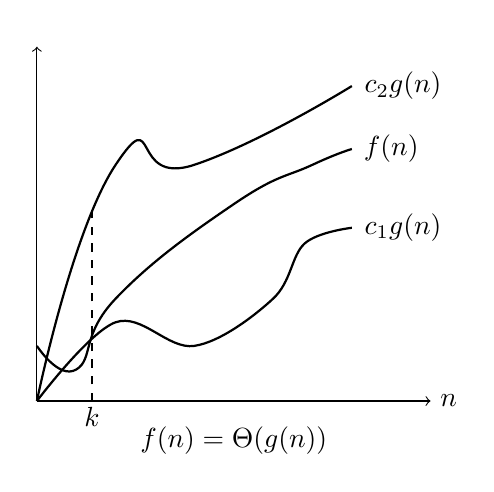
\begin{tikzpicture}
        % Axes
        \draw[->] (0,0) -- (5,0) node[right] {$n$};
        \draw[->] (0,0) -- (0,4.5) node[above] {};
        
        % Dashed line for n0
        \draw[dashed] (0.7,0) -- (0.7,2.5) node[below,yshift=-70pt] {$k$};

        % Plot for c1 * g(n) (lower bound) - Increase squiggles by lowering tension
        \draw[thick] plot[smooth, tension=0.6] coordinates {(0,0) (1,1) (2,0.7) (3, 1.3) (3.4, 2) (4,2.2)};
        \node at (4.65,2.2) {$c_1 g(n)$};

        % Plot for c2 * g(n) (upper bound) - Reduce squiggles by raising tension
        \draw[thick] plot[smooth, tension=1.0] coordinates {(0,0) (1,3) (2,3) (4,4)};
        \node at (4.65,4) {$c_2 g(n)$};

        % Plot for f(n) in between c1 g(n) and c2 g(n) - Fine-tuned squiggles by adjusting control points
        \draw[thick] plot[smooth, tension=0.8] coordinates {(0,0.7) (0.5,0.4) (1,1.3) (2.5,2.5) (3.5,3) (4,3.2)};
        \node at (4.5,3.2) {$f(n)$};
        
        % Label for Theta notation
        \node at (2.5,-0.5) {$f(n) = \Theta(g(n))$};
    \end{tikzpicture}
    \caption{Illustration af \(\Theta\)-notation, hvor \( f(n) \) er afgrænset af \( c_1 g(n) \) og \( c_2 g(n) \)}
    \label{fig:theta_notation}
\end{figure}

Figur \ref{fig:theta_notation} illustrerer $\Theta$-notation: Efter en passende tærskel $k$ er $f(n)$ begrænset nedadtil og opadtil af positive konstante multipla af $g(n)$. Figuren viser én mulig tærskel, ikke nødvendigvis den mindste. Theta beskriver den asymptotiske vækst af den funktion $f$, der er valgt. Mere kortfattet:

\[
f(n)=\Theta(g(n)): \quad f \text { vokser lige så hurtigt som } g
\]

\begin{example}

    Fra diskussionen ovenfor har vi $f(n)=3.5 n^2+4 n+36=\Theta\left(n^2\right)$, da
    \[
    3.5 n^2 \leq f(n)=3.5 n^2+4 n+36 \leq 3.5 n^2+4 n^2+36 n^2=43.5 n^2,
    \]

gælder for alle $n \geq 1$. Altså er $f(n)=\Theta\left(n^2\right)$ ifølge definition \ref{def:theta_notation} med $c_1=3.5$ og $c_2=43.5$.
\end{example}

Følgende egenskaber gælder for $\Theta$-notation:

\begin{itemize}
    \item Hvis $f(n) = \Theta(g(n))$, så er $g(n) = \Theta(f(n))$.
    \item Hvis $f(n) = \Theta(g(n))$ og $g(n) = \Theta(h(n))$, så er $f(n) = \Theta(h(n))$.
\end{itemize}

Desuden giver følgende proposition en bekvem måde at vise, at to funktioner har samme
vækstorden.

\begin{proposition} \label{prop:limit_theorem}
    Lad $f(n)$ og $g(n)$ være to ikkenegative funktioner, og antag, at der findes en konstant $c>0$, så
    \medskip
    \[
    \lim _{n \rightarrow \infty} \frac{f(n)}{g(n)}=c
    \]
    \medskip
    Da er $f(n)=\Theta(g(n))$. Hvis grænseværdien
    \medskip
    \[
    \lim _{n \rightarrow \infty} \frac{f(n)}{g(n)}
    \]
    \medskip
    desuden eksisterer, men \textbf{ikke} er lig med en positiv konstant, så er $f(n) \neq \Theta(g(n))$.
\end{proposition}

\begin{example}
    Brug proposition \ref{prop:limit_theorem} til at bevise, at hvis $f(n)=3 n^2+6 n+7$, så er $f(n)=\Theta\left(n^2\right)$. Med andre ord har $f(n)$ kvadratisk vækst.
\end{example}

\begin{solution}Lad $g(n) = n^2$. Ifølge proposition \ref{prop:limit_theorem} skal vi beregne grænseværdien:
    
    \[
    \lim_{n \to \infty} \frac{f(n)}{g(n)} = \lim_{n \to \infty} \frac{3n^2 + 6n + 7}{n^2}.
    \]
    
    Ved at dividere hvert led i tælleren med $n^2$ får vi:
    \[
    \lim_{n \to \infty} \frac{3n^2}{n^2} + \frac{6n}{n^2} + \frac{7}{n^2} = \lim_{n \to \infty} \left( 3 + \frac{6}{n} + \frac{7}{n^2} \right).
    \]
    
    Når $n \to \infty$, går leddene $\frac{6}{n}$ og $\frac{7}{n^2}$ mod $0$, så vi har:
    \[
    \lim_{n \to \infty} \frac{f(n)}{g(n)} = 3.
    \]
    
    Da denne grænseværdi er en positiv konstant ($c = 3 > 0$), følger det af proposition \ref{prop:limit_theorem}, at $f(n) = \Theta(n^2)$.
    
    Vi har dermed vist, at $f(n) = 3n^2 + 6n + 7$ har kvadratisk vækst, som ønsket.
    \end{solution}
    

\subsection*{Øvre og nedre grænse}

Antag, at vi definerer en funktion \( f(n) \) således:

\[
f(n) = 
\begin{cases} 
2n & \text{hvis } n \text{ er lige} \\ 
3n^2 & \text{hvis } n \text{ er ulige} 
\end{cases}
\]

Hvad er vækstraten for \( f(n) \)? Vi kan desværre ikke blot kategorisere \( f(n) \) som havende enten lineær eller kvadratisk vækst. Det skyldes, at grænseværdierne

\[
\lim_{n \rightarrow \infty} \frac{f(n)}{n}
\]

og

\[
\lim_{n \rightarrow \infty} \frac{f(n)}{n^2}
\]

ikke eksisterer, da \( f(n) \) hele tiden veksler mellem lineær og kvadratisk opførsel og skifter fra kvadratisk vækst til lineær vækst og tilbage igen. Det bedste, vi kan gøre, er derfor at fastlægge øvre og nedre grænser for \( f(n) \).

\textbf{For store $\mathcal{O}$: }\( f(n) = \mathcal{O}(g(n)) \), hvis \( f(n) \) ikke vokser hurtigere end \( g(n) \). Med andre ord gælder \( f(n) \leq c \cdot g(n) \) for en konstant \( c > 0 \) og for alle \( n \geq k \), hvor \( k \geq 0 \) er en konstant.

\textbf{For store Omega:} \( f(n) = \Omega(g(n)) \), hvis \( f(n) \) vokser mindst lige så hurtigt som \( g(n) \). Det vil sige, at \( f(n) \geq c \cdot g(n) \) for en konstant \( c > 0 \) og for alle \( n \geq k \), hvor \( k \geq 0 \) er en konstant.

Ud fra disse definitioner finder vi, at \( f(n) = \mathcal{O}(n^2) \) og \( f(n) = \Omega(n) \). Vi formaliserer disse overvejelser i de følgende afsnit.

\subsection*{Store \texorpdfstring{$\mathcal{O}$}{O}-notation}
Store $\mathcal{O}$-notation giver en \textit{asymptotisk øvre grænse} for en funktions vækstrate. Den anvendes ofte på en køretidsfunktion for værste tilfælde, men store $\mathcal{O}$ betyder ikke i sig selv værste tilfælde.

\begin{definition}{Store $\mathcal{O}$}
    $f(n)$ er $\mathcal{O}(g(n))$, hvis der findes positive konstanter $c$ og $k$, så der for alle $n \geq k$ gælder
    \medskip
    \[
    f(n) \leq c \cdot g(n)
    \]
    \medskip
    Det betyder, at $f(n)$ asymptotisk er begrænset opadtil af $g(n)$, dvs. at $f(n)$ højst vokser lige så hurtigt som $g(n)$, når $n$ bliver tilstrækkeligt stor.
    \label{def:big_o_notation}
\end{definition}

Udtrykket »$n$ bliver tilstrækkeligt stor« betyder, at uligheden ikke behøver at gælde for alle $n \geq 0$, men for alle $n \geq k$, hvor $k$ er en konstant. Ofte har vi ikke brug for den præcise værdi af $k$, så vi skriver »tilstrækkeligt stor«, når den præcise værdi er uden betydning.

\begin{figure}[htbp]
    \centering
    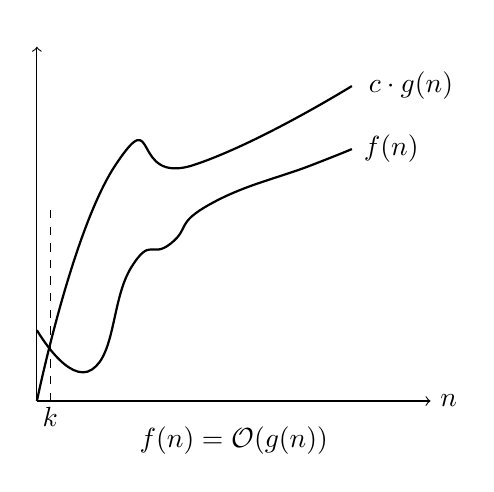
\begin{tikzpicture}
        % Axes
        \draw[->] (0,0) -- (5,0) node[right] {$n$};
        \draw[->] (0,0) -- (0,4.5) node[above] {};

        % Dashed line for n0
        \draw[dashed] (0.17,0) -- (0.17,02.5) node[below, yshift=-70pt] {$k$};

        % Plot for c * g(n) (upper bound)
        \draw[thick] plot[smooth, tension=1.0] coordinates {(0,0) (1,3) (2,3) (4,4)};
        \node at (4.75,4) {$c \cdot g(n)$};

        % Plot for f(n) below c * g(n)
        \draw[thick] plot[smooth, tension=0.9] coordinates {(0,0.9) (0.7,0.4) (1.2,1.7)  (1.7,2) (2.2,2.5) (3.5,3) (4,3.2)};
        \node at (4.5,3.2) {$f(n)$};
        
        % Label for Big O notation
        \node at (2.5,-0.5) {$f(n) = \mathcal{O}(g(n))$};
    \end{tikzpicture}
    \caption{Illustration af \(\mathcal{O}\)-notation, hvor $f(n)$ er begrænset opadtil af $c \cdot g(n)$.}
    \label{fig:big_o_notation}
\end{figure}

Figur \ref{fig:big_o_notation} illustrerer, at $f(n)$ fra et vist punkt er begrænset opadtil af $c\,g(n)$. Mere kortfattet:

\[
f(n)=\mathcal{O}(g(n)): \quad f \text{ vokser højst lige så hurtigt som } g
\]


\begin{example}
    Brug definition \ref{def:big_o_notation} til at vise, at $f(n)=3n^2+6n+7$ er $\mathcal{O}(n^2)$. Med andre ord har $f(n)$ højst kvadratisk vækst.
\end{example}

\begin{solution}
    Lad $g(n) = n^2$. Vi skal finde konstanter $c > 0$ og $k$, så $f(n) \leq c \cdot g(n)$ for alle $n \geq k$.
    
    Vi kan skrive:
    \[
    f(n) = 3n^2 + 6n + 7 \leq 3n^2 + 6n^2 + 7n^2 = 16n^2.
    \]
    Her opfylder $c = 16$ og $k = 1$ uligheden, så vi konkluderer, at $f(n) = \mathcal{O}(n^2)$.
\end{solution}

Følgende egenskaber gælder for $\mathcal{O}$-notation:
\begin{itemize}
    \item Hvis $f(n) = \mathcal{O}(g(n))$ og $g(n) = \mathcal{O}(h(n))$, så er $f(n) = \mathcal{O}(h(n))$.
    \item Konstante funktioner er $\mathcal{O}(1)$, dvs. at deres vækst er begrænset uanset inputstørrelsen.
\end{itemize}

\subsection*{Omega-notation (\texorpdfstring{$\Omega$}{Omega})}

Omega-notation giver en \textit{asymptotisk nedre grænse} for vækstraten af en bestemt funktion. Den kan anvendes på køretidsfunktioner for bedste, gennemsnitlige eller værste tilfælde; Omega betyder ikke i sig selv bedste tilfælde. \newpage

\begin{definition}{Omega-notation}\label{def:omega_notation}
    $f(n)$ er $\Omega(g(n))$, hvis der findes positive konstanter $c$ og $k$, så der for alle $n \geq k$ gælder
    \medskip
    \[
    f(n) \geq c \cdot g(n)
    \]
    \medskip
    Det betyder, at $f(n)$ asymptotisk er begrænset nedadtil af $g(n)$, dvs. at $f(n)$ vokser mindst lige så hurtigt som $g(n)$, når $n$ bliver tilstrækkeligt stor.
\end{definition}

Formuleringen »$n$ bliver tilstrækkeligt stor« angiver, at ovenstående ulighed ikke behøver at gælde for alle $n \geq 0$, men kun for $n \geq k$ for en konstant $k$. 

\begin{figure}[htbp]
    \centering
    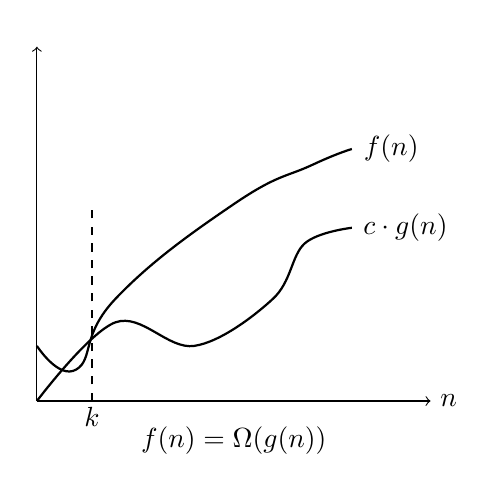
\begin{tikzpicture}
        % Axes
        \draw[->] (0,0) -- (5,0) node[right] {$n$};
        \draw[->] (0,0) -- (0,4.5) node[above] {};

        % Dashed line for n0
        \draw[dashed] (0.7,0) -- (0.7,2.5) node[below, yshift=-70pt] {$k$};

        % Plot for c * g(n) (lower bound)
        \draw[thick] plot[smooth, tension=0.6] coordinates {(0,0) (1,1) (2,0.7) (3, 1.3) (3.4, 2) (4,2.2)};
        \node at (4.68,2.2) {$c \cdot g(n)$};

        % Plot for f(n) above c * g(n)
        \draw[thick] plot[smooth, tension=0.8] coordinates {(0,0.7) (0.5,0.4) (1,1.3) (2.5,2.5) (3.5,3) (4,3.2)};
        \node at (4.5,3.2) {$f(n)$};
        
        % Label for Omega notation
        \node at (2.5,-0.5) {$f(n) = \Omega(g(n))$};
    \end{tikzpicture}
    \caption{Illustration af \(\Omega\)-notation, der viser, at $f(n)$ asymptotisk er begrænset nedadtil af $c \cdot g(n)$ for store værdier af $n$.}
    \label{fig:omega_notation}
\end{figure}

Figur \ref{fig:omega_notation} illustrerer, at $f(n)$ fra et vist punkt er begrænset nedadtil af $c\,g(n)$. Mere kortfattet:

\[
f(n)=\Omega(g(n)): \quad f \text{ vokser mindst lige så hurtigt som } g
\]


\begin{example}
    Brug definition \ref{def:omega_notation} til at vise, at $f(n)=3n^2+6n+7$ er $\Omega(n^2)$. Med andre ord har $f(n)$ mindst kvadratisk vækst.
\end{example}

\begin{solution}
    Lad $g(n) = n^2$. Vi skal finde konstanter $c > 0$ og $k$, så $f(n) \geq c \cdot g(n)$ for alle $n \geq k$.

    Vi kan skrive:
    \[
    f(n) = 3n^2 + 6n + 7 \geq 3n^2.
    \]
    Her opfylder $c = 3$ og $k = 1$ uligheden, så vi konkluderer, at $f(n) = \Omega(n^2)$.
\end{solution}

Følgende egenskaber gælder for $\Omega$-notation:
\begin{itemize}
    \item Hvis $f(n) = \Omega(g(n))$ og $g(n) = \Omega(h(n))$, så er $f(n) = \Omega(h(n))$.
    \item Positive konstante funktioner er $\Omega(1)$, dvs. at de har en nedre grænse, der ikke afhænger af inputstørrelsen.
\end{itemize}


Formelt gælder $T(n) = \Omega(g(n))$, hvis der findes konstanter $c > 0$ og $k \geq 0$, så $T(n) \geq c \cdot g(n)$ for alle $n \geq k$.

Hvis en sorteringsalgoritme for eksempel altid kræver mindst $n \log n$ sammenligninger, kan vi sige, at den har tidskompleksiteten $\Omega(n \log n)$.

\begin{example}

    Antag, at $f(n)$ er defineret som følger.
    
    \[
    f(n)= \begin{cases}2 n^{2.1} \log ^3 n & \text { hvis } n \bmod 3=0 \\ 10 n^2 \log ^{50} n & \text { hvis } n \bmod 3=1 \\ 6 n^2 \bigl(\log(n^{80})\bigr)^{30} & \text { hvis } n \bmod 3=2\end{cases}
    \]
    
    
    Angiv en øvre grænse med store $\mathcal{O}$ og en nedre grænse med store $\Omega$ for $f(n)$.
    \end{example}
    
    \begin{solution}
        For at finde en øvre grænse med store $\mathcal{O}$ og en nedre grænse med store $\Omega$ for funktionen undersøger vi hvert tilfælde. Til den øvre grænse vælger vi det led, der vokser hurtigst, når \( n \to \infty \), og til den nedre grænse det led, der vokser langsomst.
        
        \textbf{Bestem den øvre grænse med store $\mathcal{O}$}
        
        For at finde en øvre grænse med store $\mathcal{O}$ leder vi efter den gren, der har den højeste vækstrate. Leddet \(n^{2.1}\log^3 n\) dominerer til sidst både \(n^2\log^{50}n\) og \(n^2(\log n)^{30}\).
        
        En øvre grænse med store $\mathcal{O}$ for \( f(n) \) er dermed:
        \[
        f(n) = \mathcal{O}(n^{2.1} \log^3 n).
        \]
        
        \textbf{Bestem den nedre grænse med store $\Omega$}
        
        For en nedre grænse med store $\Omega$ leder vi efter den gren, der har den laveste vækstrate. Da $\log(n^{80})=80\log n$, vokser den tredje gren som et konstant multiplum af \(n^2(\log n)^{30}\), hvilket er langsommere end \(n^2(\log n)^{50}\).
        
        En nedre grænse med store $\Omega$ for \( f(n) \) er derfor:
        \[
        f(n) = \Omega(n^2 \log^{30} n).
        \]
        
        Sammenfattende har vi:
        \[
        f(n) = \mathcal{O}(n^{2.1} \log^3 n) \quad \text{og} \quad f(n) = \Omega(n^2 \log^{30} n).
        \]\end{solution}

Kort opsummeret:
\begin{itemize}
    \item Store $\mathcal{O}$-notation giver en asymptotisk øvre grænse.
    \item Omega-notation ($\Omega$) giver en asymptotisk nedre grænse.
    \item Theta-notation ($\Theta$) giver en stram asymptotisk grænse.
\end{itemize}

Når vi forstår disse notationer, får vi et mere fuldstændigt billede af en algoritmes effektivitet i forskellige scenarier.

\section{Videre analyse}
Ikke alle funktioner kan uden videre klassificeres med notationerne store $\mathcal{O}$, Omega ($\Omega$) og Theta ($\Theta$). I nogle tilfælde er en funktions vækstrate ikke let at bestemme, eller funktionen passer ikke pænt ind i en af disse kategorier. I sådanne tilfælde kan vi bruge yderligere værktøjer til at analysere funktioners vækstrate mere præcist.

\subsection*{Lille \texorpdfstring{$o$}{o}-notation}
Lille $o$-notation giver en \textit{streng øvre grænse} for en funktions vækstrate. Den beskriver en situation, hvor funktionen vokser langsommere end en anden funktion. Notationen er nyttig til at angive, at en algoritmes tidskompleksitet er strengt mindre end en given funktion.

\begin{definition}{Lille $o$}\label{def:little_o_notation}
    $f(n)$ er $o(g(n))$, hvis der for enhver positiv konstant $\epsilon > 0$ findes en konstant $k \geq 0$, så der for alle $n \geq k$ gælder
    \medskip
    \[
    f(n) < \epsilon \cdot g(n)
    \]
    \medskip
    Det betyder, at $f(n)$ vokser strengt langsommere end $g(n)$, når $n$ bliver tilstrækkeligt stor.
    
\end{definition}

Formuleringen »$n$ bliver tilstrækkeligt stor« angiver, at ovenstående ulighed ikke behøver at gælde for alle $n \geq 0$, men kun for $n \geq k$ for en konstant $k$.

\begin{figure}[htbp]
    \centering
    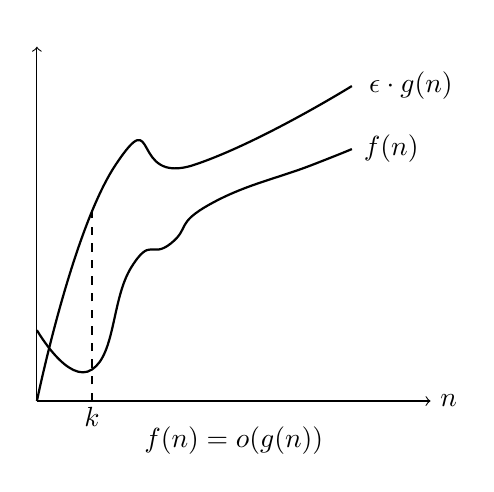
\begin{tikzpicture}
        % Axes
        \draw[->] (0,0) -- (5,0) node[right] {$n$};
        \draw[->] (0,0) -- (0,4.5) node[above] {};

        % Dashed line for n0
        \draw[dashed] (0.7,0) -- (0.7,2.5) node[below, yshift=-70pt] {$k$};

        % Plot for epsilon * g(n) (upper bound)
        \draw[thick] plot[smooth, tension=1.0] coordinates {(0,0) (1,3) (2,3) (4,4)};
        \node at (4.75,4) {$\epsilon \cdot g(n)$};

        % Plot for f(n) below epsilon * g(n)
        \draw[thick] plot[smooth, tension=0.9] coordinates {(0,0.9) (0.7,0.4) (1.2,1.7)  (1.7,2) (2.2,2.5) (3.5,3) (4,3.2)};
        \node at (4.5,3.2) {$f(n)$};
        
        % Label for Little o notation
        \node at (2.5,-0.5) {$f(n) = o(g(n))$};
    \end{tikzpicture}
    \caption{$o$-notation: $f(n)$ er strengt begrænset opadtil af $\epsilon \cdot g(n)$ for store $n$.}
    \label{fig:little_o_notation}
\end{figure}

Figur \ref{fig:little_o_notation} viser begrebet lille $o$-notation og illustrerer, at $f(n)$ er strengt begrænset opadtil af $\epsilon \cdot g(n)$. Notationen giver en streng øvre grænse for en algoritmes køretid og beskriver den asymptotiske vækstrate af algoritmens køretid på en mere præcis måde. Eller sagt mere kortfattet:

\[
f(n)=o(g(n)): \quad f \text{ vokser strengt langsommere end } g
\]

\begin{example}
    Brug definition \ref{def:little_o_notation} til at vise, at $f(n)=3n^2+6n+7$ er $o(n^3)$. Med andre ord vokser $f(n)$ strengt langsommere end $n^3$.
\end{example}

\begin{solution}
    Lad $g(n) = n^3$. Vi skal vise, at der for enhver positiv konstant $\epsilon > 0$ findes en konstant $k$, så $f(n) < \epsilon \cdot g(n)$ for alle $n \geq k$.

    Vi kan skrive:
    \[
    f(n) = 3n^2 + 6n + 7 < \epsilon \cdot n^3
    \]
    for tilstrækkeligt store $n$. Ved at dividere begge sider med $n^3$ får vi:
    \[
    \frac{f(n)}{n^3} = \frac{3n^2 + 6n + 7}{n^3} = \frac{3}{n} + \frac{6}{n^2} + \frac{7}{n^3}
    \]
    Når $n \to \infty$, går højresiden mod $0$, som er mindre end enhver positiv konstant $\epsilon$. Derfor er $f(n) = o(n^3)$.
\end{solution}

Det fører os til følgende proposition

\begin{proposition} \label{prop:little_o_theorem}
    Lad \( f(n) \) og \( g(n) \) være to ikkenegative funktioner, og antag, at
    \medskip
    \[
    \lim_{n \rightarrow \infty} \frac{f(n)}{g(n)} = 0
    \]
    \medskip
    Da er \( f(n) = o(g(n)) \), dvs. at \( f(n) \) vokser strengt langsommere end \( g(n) \), når \( n \to \infty \).
\end{proposition}

\begin{example}
    Brug proposition \ref{prop:little_o_theorem} til at bevise, at hvis \( f(n) = 3n^2 + 6n + 7 \), så er \( f(n) = o(n^3) \). Med andre ord vokser \( f(n) \) strengt langsommere end \( n^3 \).

\end{example}

\begin{solution}
    
    Lad \( g(n) = n^3 \). Ifølge proposition \ref{prop:little_o_theorem} skal vi beregne grænseværdien:
    
    \[
    \lim_{n \to \infty} \frac{f(n)}{g(n)} = \lim_{n \to \infty} \frac{3n^2 + 6n + 7}{n^3}
    \]
    
    Ved at dividere hvert led i tælleren med \( n^3 \) får vi:
    
    \[
    \lim_{n \to \infty} \frac{3n^2}{n^3} + \frac{6n}{n^3} + \frac{7}{n^3} = \lim_{n \to \infty} \left( \frac{3}{n} + \frac{6}{n^2} + \frac{7}{n^3} \right)
    \]
    
    Når \( n \to \infty \), går leddene \( \frac{3}{n} \), \( \frac{6}{n^2} \) og \( \frac{7}{n^3} \) mod \( 0 \), så vi har:
    
    \[
    \lim_{n \to \infty} \frac{f(n)}{g(n)} = 0
    \]
    
    Da grænseværdien er \( 0 \), følger det af proposition \ref{prop:little_o_theorem}, at \( f(n) = o(n^3) \).
    
    Vi har dermed vist, at \( f(n) = 3n^2 + 6n + 7 \) vokser strengt langsommere end \( n^3 \), som ønsket.
\end{solution}

Følgende egenskaber gælder for $o$-notation:
\begin{itemize}
    \item Hvis $f(n) = o(g(n))$, så er $g(n) \neq o(f(n))$.
    \item Hvis $f(n) = o(g(n))$ og $g(n) = o(h(n))$, så er $f(n) = o(h(n))$.
\end{itemize}

Lille $o$-notation giver en mere præcis måde at beskrive funktioners vækstrate på, især når funktionen vokser strengt langsommere end en anden funktion. Notationen er nyttig til at angive, at en algoritmes tidskompleksitet er strengt mindre end en given funktion, og giver en mere detaljeret forståelse af algoritmens kompleksitet.

\subsection*{Lille \texorpdfstring{$\omega$}{omega}-notation}
Lille $\omega$-notation giver en \textit{streng nedre grænse} for en funktions vækstrate. Den beskriver en situation, hvor funktionen vokser hurtigere end en anden funktion. Notationen er nyttig til at angive, at en algoritmes tidskompleksitet er strengt større end en given funktion.

\begin{definition}{Lille $\omega$}\label{def:little_omega_notation}
    $f(n)$ er $\omega(g(n))$, hvis der for enhver positiv konstant $\epsilon > 0$ findes en konstant $k \geq 0$, så der for alle $n \geq k$ gælder
    \medskip
    \[
    f(n) > \epsilon \cdot g(n)
    \]
    \medskip
    Det betyder, at $f(n)$ vokser strengt hurtigere end $g(n)$, når $n$ bliver tilstrækkeligt stor.
\end{definition}

Formuleringen »$n$ bliver tilstrækkeligt stor« angiver, at ovenstående ulighed ikke behøver at gælde for alle $n \geq 0$, men kun for $n \geq k$ for en konstant $k$.

\begin{figure}[htbp]
    \centering
    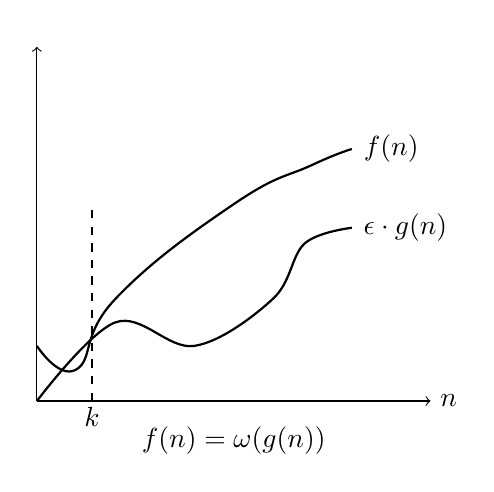
\begin{tikzpicture}
        % Axes
        \draw[->] (0,0) -- (5,0) node[right] {$n$};
        \draw[->] (0,0) -- (0,4.5) node[above] {};

        % Dashed line for n0
        \draw[dashed] (0.7,0) -- (0.7,2.5) node[below, yshift=-70pt] {$k$};

        % Plot for epsilon * g(n) (lower bound)
        \draw[thick] plot[smooth, tension=0.6] coordinates {(0,0) (1,1) (2,0.7) (3, 1.3) (3.4, 2) (4,2.2)};
        \node at (4.68,2.2) {$\epsilon \cdot g(n)$};

        % Plot for f(n) above epsilon * g(n)
        \draw[thick] plot[smooth, tension=0.8] coordinates {(0,0.7) (0.5,0.4) (1,1.3) (2.5,2.5) (3.5,3) (4,3.2)};
        \node at (4.5,3.2) {$f(n)$};
        
        % Label for Little omega notation
        \node at (2.5,-0.5) {$f(n) = \omega(g(n))$};
    \end{tikzpicture}
    \caption{$\omega$-notation: $f(n)$ er strengt begrænset nedadtil af $\epsilon \cdot g(n)$ for store $n$.}
    \label{fig:little_omega_notation}
\end{figure}

Figur \ref{fig:little_omega_notation} viser begrebet lille $\omega$-notation og illustrerer, at $f(n)$ er strengt begrænset nedadtil af $\epsilon \cdot g(n)$. Notationen giver en streng nedre grænse for en algoritmes køretid og beskriver den asymptotiske vækstrate af algoritmens køretid på en mere præcis måde. Eller sagt mere kortfattet:

\[
f(n)=\omega(g(n)): \quad f \text{ vokser strengt hurtigere end } g
\]

\begin{example}
    Brug definition \ref{def:little_omega_notation} til at vise, at $f(n)=n^3 + 6n + 7$ er $\omega(n^2)$. Med andre ord vokser $f(n)$ strengt hurtigere end $n^2$.
\end{example}

\begin{solution}
    Lad $g(n) = n^2$. Vi skal vise, at der for enhver positiv konstant $\epsilon > 0$ findes en konstant $k$, så $f(n) > \epsilon \cdot g(n)$ for alle $n \geq k$.

    Vi kan skrive:
    \[
    f(n) = n^3 + 6n + 7 > \epsilon \cdot n^2
    \]
    for tilstrækkeligt store $n$. Ved at dividere begge sider med $n^2$ får vi:
    \[
    \frac{f(n)}{n^2} = \frac{n^3 + 6n + 7}{n^2} = n + \frac{6}{n} + \frac{7}{n^2}
    \]
    Når $n \to \infty$, går højresiden mod uendelig og overstiger derfor til sidst enhver positiv konstant $\epsilon$. Altså er $f(n) = \omega(n^2)$.
\end{solution}

Det fører os til følgende proposition:

\begin{proposition} \label{prop:little_omega_theorem}
    Lad \( f(n) \) og \( g(n) \) være to ikkenegative funktioner, og antag, at
    \medskip
    \[
    \lim_{n \rightarrow \infty} \frac{f(n)}{g(n)} = \infty
    \]
    \medskip
    Da er \( f(n) = \omega(g(n)) \), dvs. at \( f(n) \) vokser strengt hurtigere end \( g(n) \), når \( n \to \infty \).
\end{proposition}

\begin{example}
    Brug proposition \ref{prop:little_omega_theorem} til at bevise, at hvis \( f(n) = n^3 + 6n + 7 \), så er \( f(n) = \omega(n^2) \). Med andre ord vokser \( f(n) \) strengt hurtigere end \( n^2 \).
\end{example}

\begin{solution}
    Lad \( g(n) = n^2 \). Ifølge proposition \ref{prop:little_omega_theorem} skal vi beregne grænseværdien:
    
    \[
    \lim_{n \to \infty} \frac{f(n)}{g(n)} = \lim_{n \to \infty} \frac{n^3 + 6n + 7}{n^2}
    \]
    
    Ved at dividere hvert led i tælleren med \( n^2 \) får vi:
    
    \[
    \lim_{n \to \infty} \frac{n^3}{n^2} + \frac{6n}{n^2} + \frac{7}{n^2} = \lim_{n \to \infty} \left( n + \frac{6}{n} + \frac{7}{n^2} \right)
    \]
    
    Når \( n \to \infty \), går leddet \( n \) mod \( \infty \), så vi har:
    
    \[
    \lim_{n \to \infty} \frac{f(n)}{g(n)} = \infty
    \]
    
    Da grænseværdien er \( \infty \), følger det af proposition \ref{prop:little_omega_theorem}, at \( f(n) = \omega(n^2) \).
    
    Vi har dermed vist, at \( f(n) = n^3 + 6n + 7 \) vokser strengt hurtigere end \( n^2 \), som ønsket.
\end{solution}

Følgende egenskaber gælder for $\omega$-notation:
\begin{itemize}
    \item Hvis $f(n) = \omega(g(n))$, så er $g(n) \neq \omega(f(n))$.
    \item Hvis $f(n) = \omega(g(n))$ og $g(n) = \omega(h(n))$, så er $f(n) = \omega(h(n))$.
\end{itemize}


Lille $\omega$-notation giver en mere præcis måde at beskrive funktioners vækstrate på, især når funktionen vokser strengt hurtigere end en anden funktion. Notationen er nyttig til at angive, at en algoritmes tidskompleksitet er strengt større end en given funktion, og giver en mere detaljeret forståelse af algoritmens kompleksitet. 

\subsection*{Brug af lille \texorpdfstring{$o$}{o} og lille \texorpdfstring{$\omega$}{omega} til at bestemme \texorpdfstring{$\mathcal{O}$}{O} og \texorpdfstring{$\Omega$}{Omega}}
Notationerne lille $o$ og lille $\omega$ kan bruges til at give mere præcise grænser, når vi bestemmer store $\mathcal{O}$ og $\Omega$. De hjælper med at afgøre, om en funktion vokser strengt langsommere eller strengt hurtigere end en anden funktion, hvilket kan være nyttigt i asymptotisk analyse.

\begin{example}
    Se på funktionen \( f(n) = n^2 + 3n + 2 \). Vi vil bestemme store $\mathcal{O}$ og $\Omega$.

    \begin{enumerate}
        \item \textbf{Store $\mathcal{O}$-notation:}
        
        For at bestemme store $\mathcal{O}$ ser vi på forholdet \( \frac{f(n)}{g(n)} \), hvor \( g(n) = n^2 \). Ved hjælp af proposition \ref{prop:big_o_theorem} beregner vi \(\limsup\)\footnote{Notationen \(\limsup\) står for »limes superior« (øvre grænseværdi) og betragter den øvre grænse for værdierne af forholdet $\frac{f(n)}{g(n)}$, når $n$ vokser. I modsætning til en almindelig grænseværdi, som ikke nødvendigvis eksisterer, hvis funktionen oscillerer, eksisterer \(\limsup\) altid for reelle følger og indfanger den maksimale vækstopførsel i det lange løb.}:
        \[
        \limsup_{n \to \infty} \frac{f(n)}{g(n)} = \limsup_{n \to \infty} \frac{n^2 + 3n + 2}{n^2} = \limsup_{n \to \infty} \left( 1 + \frac{3}{n} + \frac{2}{n^2} \right).
        \]
        Når \( n \to \infty \), går leddene \( \frac{3}{n} \) og \( \frac{2}{n^2} \) mod \( 0 \), så:
        \[
        \limsup_{n \to \infty} \frac{f(n)}{g(n)} = 1.
        \]
        Da denne værdi er endelig, konkluderer vi, at \( f(n) = \mathcal{O}(n^2) \).

        \item \textbf{Store $\Omega$-notation:}
        
        For at bestemme store $\Omega$ beregner vi \(\liminf\) af det samme forhold\footnote{Notationen \(\liminf\) står for »limes inferior« (nedre grænseværdi) og betragter den nedre grænse for værdierne af forholdet $\frac{f(n)}{g(n)}$, når $n$ vokser. I modsætning til en almindelig grænseværdi, som ikke nødvendigvis eksisterer, hvis funktionen oscillerer, eksisterer \(\liminf\) altid for reelle følger. Den indfanger den minimale vækstopførsel på lang sigt og fremhæver den laveste hastighed, hvormed $f(n)$ vokser i forhold til $g(n)$, når $n$ bliver stor.}:
        \[
        \liminf_{n \to \infty} \frac{f(n)}{g(n)} = \liminf_{n \to \infty} \frac{n^2 + 3n + 2}{n^2} = \liminf_{n \to \infty} \left( 1 + \frac{3}{n} + \frac{2}{n^2} \right).
        \]
        Igen går leddene \( \frac{3}{n} \) og \( \frac{2}{n^2} \) mod \( 0 \), når \( n \to \infty \), så:
        \[
        \liminf_{n \to \infty} \frac{f(n)}{g(n)} = 1.
        \]
        Da denne værdi er positiv, konkluderer vi, at \( f(n) = \Omega(n^2) \).
    \end{enumerate}

    Sammenfattende har vi:
    \[
    f(n) = \mathcal{O}(n^2) \quad \text{og} \quad f(n) = \Omega(n^2).
    \]
\end{example}

        Ved at bruge notationerne lille $o$ og lille $\omega$ kan vi give mere præcise grænser for store $\mathcal{O}$ og $\Omega$, hvilket hjælper os til bedre at forstå funktioners vækstrater og algoritmers kompleksitet. Men måske endnu vigtigere kan vi bruge grænseværdibegrebet til at bestemme store $\mathcal{O}$ og $\Omega$ ud fra lille $o$ og lille $\omega$.

        Det fører os til følgende propositioner:

        \begin{proposition} \label{prop:big_o_theorem}
            Lad \( f(n) \) og \( g(n) \) være to ikkenegative funktioner med $g(n)>0$ for alle tilstrækkeligt store $n$. Hvis
            \medskip
            \[
            \limsup_{n \rightarrow \infty} \frac{f(n)}{g(n)} < \infty
            \]
            \medskip
            så er \( f(n) = \mathcal{O}(g(n)) \), dvs. at \( f(n) \) asymptotisk højst vokser lige så hurtigt som \( g(n) \).
        \end{proposition}
        
        Og desuden:


        \begin{proposition} \label{prop:big_omega_theorem}
            Lad \( f(n) \) og \( g(n) \) være to ikkenegative funktioner med $g(n)>0$ for alle tilstrækkeligt store $n$. Hvis
            \medskip
            \[
            \liminf_{n \rightarrow \infty} \frac{f(n)}{g(n)} > 0
            \]
            \medskip
            så er \( f(n) = \Omega(g(n)) \), dvs. at \( f(n) \) asymptotisk vokser mindst lige så hurtigt som \( g(n) \).
        \end{proposition}
        
        Disse propositioner giver en mere formel måde at bestemme store $\mathcal{O}$ og $\Omega$ ud fra lille $o$ og lille $\omega$. Ved at undersøge grænseværdierne af forholdet mellem funktioner kan vi afgøre, om en funktion højst eller mindst vokser lige så hurtigt som en anden funktion, hvilket giver en mere stringent analyse af vækstrater.
            
            \begin{example}
            Brug proposition \ref{prop:big_omega_theorem} til at bevise, at hvis \( f(n) = 3n^2 + 5n + 7 \), så er \( f(n) = \Omega(n^2) \).
            \end{example}
            
            \begin{solution}
            Lad \( g(n) = n^2 \). Vi skal beregne den nedre grænseværdi (lim inf) af \( \frac{f(n)}{g(n)} \), når \( n \) går mod uendelig:
            
            \[
            \liminf_{n \to \infty} \frac{f(n)}{g(n)} = \liminf_{n \to \infty} \frac{3n^2 + 5n + 7}{n^2}.
            \]
            
            Ved at dividere hvert led i tælleren med \( n^2 \) har vi:
            \[
            = \liminf_{n \to \infty} \left( 3 + \frac{5}{n} + \frac{7}{n^2} \right).
            \]
            
            Når \( n \to \infty \), går leddene \( \frac{5}{n} \) og \( \frac{7}{n^2} \) mod \( 0 \). Dermed får vi:
            \[
            \liminf_{n \to \infty} \frac{f(n)}{g(n)} = 3.
            \]
            
            Da denne grænseværdi er en positiv konstant \( c = 3 > 0 \), følger det af proposition \ref{prop:big_omega_theorem}, at \( f(n) = \Omega(n^2) \). Eksemplet viser, at \( f(n) = 3n^2 + 5n + 7 \) har kvadratisk vækst i betydningen nedre grænse. \end{solution}

            \begin{example}
                Afgør, om \( f(n) = 2n \sin(n) + 3n \) er \( \mathcal{O}(n) \) og \( \Omega(n) \), ved at bruge grænseværdierne som beskrevet i propositionerne \ref{prop:big_o_theorem} og \ref{prop:big_omega_theorem}. \end{example}
                
                \begin{solution}
                Lad \( g(n) = n \). Vi undersøger opførslen af \( \frac{f(n)}{g(n)} \), når \( n \to \infty \).
                
                Først udtrykker vi \( \frac{f(n)}{g(n)} \) således:
                \[
                \frac{f(n)}{g(n)} = \frac{2n \sin(n) + 3n}{n} = 2 \sin(n) + 3.
                \]
                
                Nu analyserer vi grænseværdiens opførsel, når \( n \to \infty \):
                \[
                \frac{f(n)}{g(n)} = 2 \sin(n) + 3.
                \]
                
                Da \( \sin(n) \) svinger mellem \( -1 \) og \( 1 \), når \( n \) vokser, svinger udtrykket \( 2 \sin(n) + 3 \) mellem \( 1 \) og \( 5 \). Den almindelige grænseværdi \( \lim_{n \to \infty} \frac{f(n)}{g(n)} \) eksisterer derfor ikke på grund af denne svingning.
                
                Vi kan dog beregne \(\limsup\) og \(\liminf\) af \( \frac{f(n)}{g(n)} \):
                \[
                \limsup_{n \to \infty} \frac{f(n)}{g(n)} = 5 \quad \text{og} \quad \liminf_{n \to \infty} \frac{f(n)}{g(n)} = 1.
                \]
                
                Da \(\limsup\) er endelig (\(5\)), konkluderer vi ifølge proposition \ref{prop:big_o_theorem}, at \( f(n) = \mathcal{O}(n) \). Da \(\liminf\) er positiv (\(1\)), konkluderer vi tilsvarende ifølge proposition \ref{prop:big_omega_theorem}, at \( f(n) = \Omega(n) \).
                \end{solution}
                
                
                

        \subsection*{Brug af grænseværdier til at bestemme asymptotiske notationer (en uformel fremgangsmåde)}

        En uformel, men praktisk fremgangsmåde til at bestemme store $\mathcal{O}$ og $\Omega$ består i at undersøge forholdet \( \frac{f(n)}{g(n)} \), når \( n \to \infty \). Vi har allerede set denne fremgangsmåde i propositionerne \ref{prop:limit_theorem}--\ref{prop:big_omega_theorem}. Selv om metoden ikke er lige så stringent som formelle propositioner, giver den hurtig indsigt i vækstrater.
        
        Følgende regler viser, hvordan grænseværdier kan anvendes på hver notation:
       

        \begin{custombox}{Uformel grænseværdimetode}
            \[
                \begin{array}{ll}
                \displaystyle \lim_{n \to \infty} \frac{f(n)}{g(n)} = L<\infty & \Rightarrow f(n) = \mathcal{O}(g(n)) \\[10pt]
                \displaystyle \lim_{n \to \infty} \frac{f(n)}{g(n)} = L>0 & \Rightarrow f(n) = \Omega(g(n))
                \end{array}
                \]
                \medskip
                \textbf{Bemærk:} Denne fremgangsmåde er en uformel retningslinje og ikke en streng matematisk definition. Der er tilfælde, hvor den grænseværdibaserede metode ikke kan anvendes, men den er ofte et bekvemt værktøj til at bestemme asymptotisk opførsel.
        \end{custombox}
        
        Reglerne fungerer således:
        \begin{itemize}
            \item \textbf{Store \(\mathcal{O}\):} Hvis grænseværdien eksisterer og ikke er uendelig, er \( f(n) = \mathcal{O}(g(n)) \), dvs. at \( f(n) \) ikke vokser hurtigere end \( g(n) \).
            \item \textbf{Store \(\Omega\):} Hvis grænseværdien eksisterer og er forskellig fra nul, er \( f(n) = \Omega(g(n)) \), dvs. at \( f(n) \) vokser mindst lige så hurtigt som \( g(n) \).
        \end{itemize}
        
        \begin{example}
            Afgør ved hjælp af den uformelle grænseværdimetode, om $\sqrt{n} \cdot \log n=\mathcal{O}(n \log n)$.
        \end{example}

        \begin{solution}
            Vi skal beregne grænseværdien af forholdet \( \frac{\sqrt{n} \cdot \log n}{n \log n} \), når \( n \to \infty \). Ved at forenkle udtrykket får vi:
            
            \[
            \lim_{n \to \infty} \frac{\sqrt{n} \cdot \log n}{n \log n} = \lim_{n \to \infty} \frac{\sqrt{n}}{n} = \lim_{n \to \infty} \frac{1}{\sqrt{n}} = 0.
            \]
            
            Da grænseværdien er endelig, konkluderer vi, at \( \sqrt{n} \cdot \log n = \mathcal{O}(n \log n) \). Vi bemærker også, at da grænseværdien er 0, kan vi slutte, at \( \sqrt{n} \cdot \log n \neq \Omega(n \log n) \).
            
        \end{solution}

        Grænseværdimetoden er bekvem, men ikke endegyldig. For nogle funktioner (fx oscillerende funktioner) bør de formelle definitioner og propositioner anvendes direkte. Den grænseværdibaserede teknik er en nyttig tommelfingerregel, især når den asymptotiske vækst er tydelig.
    
\subsection*{Sammenligning af notationer}
Vi afslutter kapitlet med at sammenligne de forskellige asymptotiske notationer og deres indbyrdes relationer:

\begin{enumerate}
    \item \( f(n) = \mathcal{O}(g(n)) \text{ og } f(n) = \Omega(g(n)) \Leftrightarrow f(n) = \Theta(g(n)) \)
    
    Denne relation siger, at hvis \( f(n) \) asymptotisk både er begrænset opadtil af \( g(n) \) (store \(\mathcal{O}\)) og begrænset nedadtil af \( g(n) \) (store \(\Omega\)), så vokser \( f(n) \) og \( g(n) \) lige hurtigt, hvilket betegnes \( \Theta(g(n)) \). Med andre ord vokser \( f(n) \) asymptotisk hverken hurtigere eller langsommere end \( g(n) \), når \( n \to \infty \). \medskip

    \item \( f(n) = o(g(n)) \Rightarrow f(n) = \mathcal{O}(g(n)) \)
    
    Hvis \( f(n) = o(g(n)) \), betyder det, at \( f(n) \) vokser strengt langsommere end \( g(n) \), når \( n \to \infty \). Derfor er \( f(n) \) asymptotisk begrænset opadtil af \( g(n) \), men vokser ikke lige så hurtigt, hvilket begrunder, at \( f(n) = \mathcal{O}(g(n)) \).\medskip

    \item \( f(n) = \mathcal{O}(g(n)) \Leftrightarrow g(n) = \Omega(f(n)) \)
    
    Denne ækvivalens viser den symmetriske sammenhæng mellem store \(\mathcal{O}\) og store \(\Omega\). Hvis \( f(n) \) asymptotisk er begrænset opadtil af \( g(n) \) (dvs. at \( f(n) \) ikke vokser hurtigere end \( g(n) \)), kan vi også sige, at \( g(n) \) vokser mindst lige så hurtigt som \( f(n) \) (dvs. \( g(n) = \Omega(f(n)) \)). \medskip

    \item \( f(n) = \omega(g(n)) \Rightarrow f(n) = \Omega(g(n)) \)
    
    Når \( f(n) = \omega(g(n)) \), betyder det, at \( f(n) \) vokser strengt hurtigere end \( g(n) \), når \( n \to \infty \). Da \( f(n) \) asymptotisk er større, følger det, at \( f(n) \) vokser mindst lige så hurtigt som \( g(n) \), så \( f(n) = \Omega(g(n)) \) er sand. \medskip

    \item \( f(n) = o(g(n)) \Leftrightarrow g(n) = \omega(f(n)) \)
    
    Denne ækvivalens viser den symmetriske sammenhæng mellem lille \(o\) og lille \(\omega\). Hvis \( f(n) = o(g(n)) \), dvs. at \( f(n) \) vokser strengt langsommere end \( g(n) \), kan vi også sige, at \( g(n) \) vokser strengt hurtigere end \( f(n) \), eller \( g(n) = \omega(f(n)) \). Relationen fremhæver den strenge forskel i deres vækstrater, når \( n \to \infty \).
\end{enumerate}

I dette kapitel har vi undersøgt tidskompleksitet som et middel til at vurdere algoritmers effektivitet. Vi introducerede notationerne store $\mathcal{O}$, Omega ($\Omega$) og Theta ($\Theta$) som måder at fastlægge øvre, nedre og stramme grænser for vækstrater på, hvilket hjælper os med at forstå, hvordan krav til køretid og plads skalerer med inputstørrelsen.

Vi fremhævede, hvor vigtigt det er at se bort fra konstanter og led af lavere orden i asymptotisk analyse og i stedet fokusere på det dominerende led. Desuden undersøgte vi notationerne lille $o$ og lille $\omega$ for strengere øvre og nedre grænser, som giver mere præcis indsigt i kompleksitet.

Til sidst sammenlignede vi notationerne og deres vigtigste relationer og byggede dermed et fundament for at vurdere algoritmers kompleksitet både teoretisk og praktisk -- som forberedelse til den praktiske analyse af tidskompleksitet i næste kapitel.
